
\documentclass[thesis-solanki.tex]{subfiles}

\providecommand\codeLibrary[1]{\texttt{\bfseries #1}}
\providecommand\metaSyntacticVariable[1]{\textsl{\ttfamily #1}}
\providecommand\mSV{\metaSyntacticVariable}

\begin{document}

\chapter{Prototype 1}{\label{proto1}}



\section{About this chapter}
\begin{comment}

This chapter throws light on what \progLang{Prolog} does to resolve a given query via \textit{unification} and this can be replicated in
the host language along with the challenges.

This chapter discusses the aspects of opening a language while preserving the original structure of a closed recursive structure in
\progLang{Haskell}. Also discussed are the issues related to customizing certain aspects such as meta-syntactic variables.
\end{comment}

This chapter demonstrates a fairly generic\endnote{%
  Really try to avoid hedging your bets with scare-quotes.
}
procedure of creating an open embedded domain specific language in \progLang{Haskell} along
with \textit{monadic unification}. As a proof of concept, the implementation consists of creating a \progLang{Prolog} like open language
whose unification procedure is carried out in a monad.


\section{Ideas}
There are four main ideas in this chapter\endnote{%
  The list of four components seems to be of different kinds of things.
  \begin{compactitem}
  \item Items 2 and 3 are libraries.
  \item Item 4 is what you are building
  \end{compactitem}
  Do you see the circularity of describing the thing you are building as a component of itself?
}
that we work with to develop a working implementation of embedded \progLang{Prolog}
using the concepts mentioned above.

\begin{enumerate}
\item \progLang{Prolog}

The language itself has a number of sub components.
The ones relevant to this thesis are,
\begin{enumerate}
\item Language, the syntax, semantics.

\item Database, or the knowledge base where the rules are stored.

\item Unification

\item
  \progLang{Prolog} has to satisfy a list of goals while maintaining variable bindings and choice points.
  For a non empty list of list of goals, it looks through the knowledge base for matching rules and attempts at
  unifying the terms and repeats until all goals have been satisfied.
  If more than one option is available, they are recorded as choice points which are later used for backtracking
  and finding other possible solutions.

\item
  Lastly, the query resolver which combines the unification and search strategy to return a result.\endnote{%
    Avoid starting sentences with ``And''---except where you want to be surprising.
}
\end{enumerate}

\item \codeLibrary{prolog-0.2.0.1} \cite{prolog-lib}

  One of the existing implementation of \progLang{Prolog} in \progLang{Haskell} though partial provides a starting
  point for the implementation providing certain components to exercise our approach.
  The main components of this library are adopted from \progLang{Prolog} and modified\yyy{,}{:}

\begin{enumerate}
\item the language, adopted from \progLang{Prolog} but trimmed down;

\item the database;\endnote{%
  and so on.
}

\item Unifier

\item Read-Eval-Print Loop(REPL)

\item Interpreter which consists of a parsing mechanism and resembles the query resolver.
\end{enumerate}

\item \codeLibrary{unification-fd} \cite{unification-fd-lib}

This library provides tools for first-order structural unification over general structure types along with mechanisms for a modifiable
generic unification algorithm implementation.

The relevant components are,
\begin{enumerate}
\item The \Verb!Unifiable! class

\item The \Verb!UTerm! data type

\item Variables\endnote{%
  what does this reference?
},
  \Verb!STVar!, \Verb!IntVar!

\item The \Verb!Binding! monad

\item Unification (\Verb!unify! and \Verb!unifyOccurs!)
\end{enumerate}

\item Prototype 1

  This implementation applies to practice the procedure to create an open language to accommodate types,
  custom variables, quantifiers and logic and recovering primitives while preserving the structure of a
  language commonly defined by a recursive abstract syntax tree.
  The resulting language is then adapted to apply a \progLang{Prolog} like unification.

The implementation consists of the following components,
\begin{enumerate}
\item An open language

\item Compatibility with the unification library \cite{unification-fd-lib}

\item Variable bindings\endnote{%
  Decide on a convention for capitals.
}

\item Monadic unification

\end{enumerate}
\end{enumerate}

Each of the components are discussed in the following sections.


\section{How Prolog works}

To replicate \progLang{Prolog} we look into how it works \cite{webiste:learnprolognow}.

\textcolor{red}{There's a sentence or more missing here. The sentence above leads up to expect a very
  high-level view.  Below, we are in the middle of discussing a syntax feature called terms.
  Below I would simplify, and just write ``\progLang{Prolog} has three types of terms:''.
}

As any other language\endnote{%
  Clean up the sentence!
  Do you mean ``As with any other language, we start with the syntax and semantics.''? 
  
  When we talk about a language we talk about the programming constructs may be?
}
we start with the syntax and semantics. We begin with the programming constructs of the language.

\progLang{Prolog} has three types of terms::
\begin{enumerate}
\item Constants.

\item Variables.

\item Complex terms.
\end{enumerate}

Two terms can be unified if they are the same or the variables can be assigned to terms such that the resulting
terms are equal.

The possibilities are,
\begin{enumerate}
\item If \mSV{term1} and \mSV{term2} are constants, then \mSV{term1} and \mSV{term2} unify if and only if they
  are the same atom, or the same number.
\begin{code-list}[h]
\begin{minted}[linenos]{prolog}
?-  =(mia,mia).
yes
\end{minted}
\end{code-list}

\item If \mSV{term1} is an uninstantiated variable and \mSV{term2} is any type of term, then \mSV{term1}
  and \mSV{term2} unify, and \mSV{term1} is instantiated to \mSV{term2}\,.
  Similarly, if \mSV{term2} is a variable and \mSV{term1} is any type of term, then \mSV{term1} and \mSV{term2}
  unify, and \mSV{term2} is instantiated to \mSV{term1} . (So if they are both 
variables, they’re both instantiated to each other, and we say that they share values.)
\begin{code-list}[h]
\begin{minted}[linenos]{prolog}
?-  mia  =  X.
X  =  mia
yes
\end{minted}

\begin{minted}[linenos]{prolog}
?-  X  =  Y.
yes
\end{minted}
\end{code-list}

\item If \mSV{term1} and \mSV{term2} are complex terms, then they unify if and only if:

\begin{enumerate}
\item They have the same functor and arity, and

\item all their corresponding arguments unify, and

\item the variable instantiations are compatible.
\end{enumerate}
\begin{code-list}[h]

\begin{minted}[linenos]{prolog}
?-  k(s(g),Y)  =  k(X,t(k)).
X  =  s(g)
Y  =  t(k)
yes
\end{minted}
\end{code-list}


\item Two terms unify if and only if it follows from the previous three clauses that they unify.
\end{enumerate}

Unification is just a part of the process \yyy{were}{where} the language
attempts to find a solution for the given query using the rules provided
in the knowledge base.
The other part is actually reaching a point where two terms need to be
unified i.e searching.
Together they form the query resolver in \progLang{Prolog}.

\newpage

For example, consider the append function

\begin{minted}[linenos]{prolog}
append([],L,L).
append([H|T],L2,[H|L3])  :-  append(T,L2,L3).
\end{minted}


\begin{figure}[h]
\centering
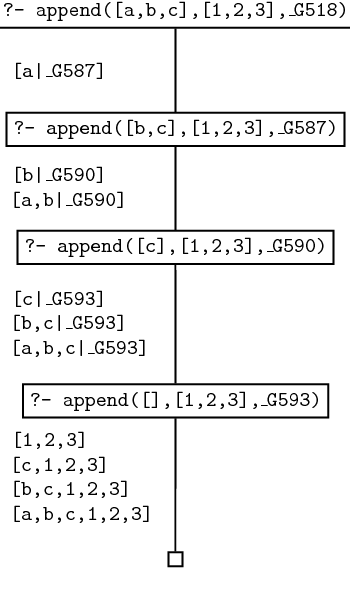
\includegraphics[scale = 0.5]{PrologAppendWorking.png}
\caption{Trace for append \cite{webiste:learnprolognowappend}}
\label{fig:Trace for append}
\end{figure}

\begin{comment}
This chapter looks into solving the issue of conflicting type systems of the languages in question. \progLang{Haskell} is a strong
statically typed language requiring type signature for programming constructs at compile time while \progLang{Prolog} is strong dynamically
typed which lets through untyped programs. This prototype throws light on the process of tackling the issues involved in creating
a data type to replicate the target language type system while conforming to the host language restrictions and also utilizing the
benefits.
\end{comment}

In this prototype we explore the unification aspect only.

\section{What we do in this Prototype}
This prototype throws light on the process of tackling the issues involved in creating
a data type to replicate the target language type system while conforming to the host language restrictions and also utilizing the
benefits.


We have a \progLang{Prolog} like language in \progLang{Haskell} defined via \textit{data}.

The language defined is recursive in nature.

We convert it into a non recursive data type.


Basically we do Unification monadically.


\section{Creating a data type}

To start we need to define a abstract syntax for the \progLang{Prolog} like language. But there is a conflict between the type systems as
we shall discuss.


A type system consists of a set of rules to define a \yyy{"}{``}type\yyy{"}{''} to different constructs in a programming language such as variables, functions
and so on. A static type system requires types to be attached to the programming constructs before hand which results in finding errors at
compile time and thus increase the reliability of the program. The other end is the dynamic type system which passes through code which
would not have worked in former environment, it comes of as less rigid.

\textcolor{red}{Why do we need the following two paragraphs? To talk about the type systems of the languages}

The advantages of static typing \cite{meijer2004static}
\begin{enumerate}
\item Earlier detection of errors
\item Better documentation in terms of type signatures
\item More opportunities for compiler optimizations
\item Increased run-time efficiency
\item Better developer tools
\end{enumerate}

For dynamic typing
\begin{enumerate}
\item Less rigid
\item Ideal for prototyping / unknown / changing requirements or unpredictable behaviour
\item Re-usability
\end{enumerate}

Since \progLang{Haskell} is statically type we would need to define a \yyy{"}{``}typed\yyy{"}{''} language which should have a
number of constructs representing different terms in \progLang{Prolog} such as complex structures (for example
predicates, clauses etc.), don't cares, cuts, variables and so on.\endnote{%
  Drop the ``would''s here.  We \textit{do} need to define a \progLang{Prolog} type.
}

Consider the language {in Figure~\ref{tab:closed-terms}} which has been adopted from
\cite{prolog-lib}.

\begin{code-list}
\begin{minted}[linenos]{haskell}
  data VariableName = VariableName Int String
  deriving (Eq, Data, Typeable, Ord)
  data Atom         = Atom      !String
                    | Operator  !String
  deriving (Eq, Ord, Data, Typeable)
  data Term = Struct Atom [Term]
            | Var VariableName
            | Wildcard
            | Cut Int
  deriving (Eq, Data, Typeable)
  data Clause = Clause { lhs :: Term, rhs_ :: [Goal] }
              | ClauseFn { lhs :: Term, fn :: [Term] -> [Goal] }
  deriving (Data, Typeable)
  type Program = [Sentence]
  type Body    = [Goal]
  data Sentence = Query   Body
                | Command Body
                | C Clause
  deriving (Data, Typeable)
\end{minted}
  \caption{A classic recursive grammar}
  \label{tab:closed-terms}
\end{code-list}

Even though \textit{Term} has a number of constructors the resulting construct has a single type. Hence, a function would still be untyped
/ singly typed,\par
\begin{minted}{haskell}
append :: [Term] -> [Term] -> [Term]
\end{minted}

\begin{comment}
The \xxx{above} data type \yyy{}{Figure~\ref{tab:closed-terms}} is recursive as seen in the constructor,
\mint{haskell}|Struct Atom [Term]|
\end{comment}

Figure~\ref{tab:closed-terms} is a classic example of using a recursive data type to define the
abstract syntax of a language.\endnote{%
  ``is a classic example of \yyy{}{using a recursive data type} \xxx{a recursive grammar} to define the
abstract syntax of a language.'' --- perhaps?
}
One of the issues with the above datatype is that it is not possible to distinguish the structure of the data from the
data type itself \cite{sheard2004two}.
Moreover, the primitives of the language\endnote{%
  What do you mean by ``primitives of the language''?
  Adopted from \cite{website:understandingalgebrasfpcomplete}
}
are not accessible as the language can have expressions of only one
type i.e.
\yyy{"}{``}Term\yyy{"}{''}.

\begin{comment}
\begin{minted}[linenos]{haskell}
type Atom         = String
data VariableName = VariableName Int String
      deriving (Eq, Data, Typeable, Ord)
data Term = Struct Atom [Term]
          | Var VariableName
          | Wildcard -- Don't cares
          | Cut Int
      deriving (Eq, Data, Typeable)
\end{minted}
Also one cannot create Quantifiers plus logic
\end{comment}

\begin{comment}
The solution \xxx{to} would be to add a type constructor split the data type into two levels, a single recursive
data type is replaced by two related data types.
\end{comment}
\endnote{%
  I cannot follow this sentence.
I do not know what I was thinking
}
Consider the code in Figure~\ref{tab:non-recurse}
\begin{code-list}
  \begin{minted}[gobble=3,linenos]{haskell}
    data FlatTerm a = Struct Atom [a]
                    | Var VariableName
                    | Wildcard
                    | Cut Int
               deriving (Show, Eq, Ord)
  \end{minted}
  \caption{A flattened (non-recursive) grammar}
  \label{tab:non-recurse}
\end{code-list}

One result of the approach is that the non-recursive type
\texttt{FlatTerm} is modular and generic as the structure
"FlatTerm"\endnote{%
  You have `\textit{FlatTerm}' and `"FlatTerm"'.  Why not \texttt{FlatTerm} or better yet
  \texttt{\csname @backslashchar\endcsname code\{FlatTerm\}}, where \texttt{\csname @backslashchar\endcsname code} is a macro you define.
}
is separate
from its\endnote{%
  Do you understand why ``it's'' should be ``its'' here?
  Yes
}
type which is \yyy{"}{``}a\yyy{"}{''}.
The above language can be of any type \textit{a}. A more accurate way of saying it would be that \textit{a} can be a \textit{kind} in
\progLang{Haskell}.\endnote{%
  Why do we explain \textit{kinds}?
  Is this in preparation for \texttt{\bfseries Functor}?
  Well Int, String etc etc are kinds in haskell so a FlatTerm int where int is *
}

In type theory, a kind is the type of a type constructor or, less commonly, the type of a higher-order type operator. A kind system is
essentially a simply typed lambda calculus 'one level up,' endowed with a primitive type, denoted * and called 'type,' which is the kind of
any (monomorphic) data type for example \cite{website:kindhaskellwiki},

\begin{minted}[linenos]{haskell}
Int :: *
Maybe :: * -> *
Maybe Bool :: *
a -> a :: *
[] :: * -> *
(->) :: * -> * -> *
\end{minted}

Simply speaking we can have something like
\mint{haskell}|FlatTerm Bool|

and a generic function like,
\mint{haskell}|function :: (a -> b) -> FlatTerm a -> FlatTerm b|
\textcolor{green}{%
  Why is this {\color{blue}\Verb|map|} rather than {\color{blue}\Verb|fmap|}\,?
  I think this is more to say all terms in the language can be (FlatTerm a) and not (FlatTerm (FlatTerm (FlatTerm ....)))
}

Although one problem remains, how does one represent infinitely nested / deep expressions of the above language, for example something of
the form,

\mint{haskell}|FlatTerm(FlatTerm (FlatTerm (FlatTerm (....... (a)))))|

and how to represent it generically to perform operations on it since,
\begin{minted}[linenos]{haskell}
(FlatTerm a) != (FlatTerm (FlatTerm a))
\end{minted}
%
because with our original grammar all the expression that could be defined would be represented by a single entity \yyy{"}{``}Term\yyy{"}{''} no matter how
infinitely deep they were.

The approach to tackling this problem is to find the \yyy{"}{``}fixed-point\yyy{"}{''}.
After infinitely many iterations we should get to a fixed point where further iterations make no
difference.
It means that applying one more ExprF would not change anything – a fix point does not move under FlatTerm.

\progLang{Haskell} provides it in two forms,\endnote{%
  Why do you need to discuss value fixed points (\textit{i.e.,} \texttt{\bfseries fix})?  Do you need them?

  Well not really but since we are talking about fixed point in general
}
\begin{enumerate}

\item The fix function in the \texttt{Control.Monad.Fix} module allows for the definition of recursive functions in \progLang{Haskell}. Consider the following scenario,

\mint{haskell}|fix :: (a -> a) -> a|

The above function results in an infinite application stream,
\mint{haskell}|f s : f (f (f (... )))|

A fixed point of a function f is a value a such that f a == a. This is where the name of fix comes from: it finds the least-defined fixed
point of a function.

\item And in type constructor form,

\mint{haskell}|newtype Fix f = f (Fix f)|

which we apply to our abstract syntax.

\end{enumerate}


The resulting language is of the form,
\begin{minted}[linenos]{haskell}
data Prolog = P (Fix FlatTerm) deriving (Show,Eq,Ord)
\end{minted}
%
simply speaking all the expressions resulting from \textit{FlatTerm} can be represented  by the type signature \textit{Fix FlatTerm}.

A sample function working with such expressions would be of the form,
\mint{haskell}|func :: Fix FlatTerm -> Fix FlatTerm|


Generically speaking, the language can be expanded for additional functionality without changing or modifying the base structure. Consider
the scenario where the language needs to accommodate additional type of terms,

\begin{enumerate}
\item Manually modifying the structure of the language, as shown in Figure~\ref{tab:man-enhan-gram}
  \begin{code-list}
    \begin{minted}[linenos,gobble=5]{haskell}
      type Atom            = String

      data VariableName    = VariableName Int String
      deriving (Eq, Data, Typeable, Ord)

      data Term  = Struct Atom [Term]
                 | Var VariableName
                 | Wildcard
                 | Cut Int
                 | New_Constructor_1 .........
                 | New_Constructor_2 .........
        deriving (Eq, Data, Typeable)
    \end{minted}
    \caption{A manually enhanced recursive grammar}
    \label{tab:man-enhan-gram}
  \end{code-list}

This would then trigger a ripple effect throughout the architecture because accommodations need to be made for the new functionality.

\item The other option would be to \textit{functorize} language like we did by adding a type variable which can be used to plug something that provides the functionality into the language.
Consider the following example,

\begin{minted}[linenos]{haskell}
data Box f = Abox | T f (Box f) deriving (.........)
\end{minted}

then something like,
\begin{minted}[linenos]{haskell}
T (Struct 'atom' [Abox, T (Cut 0)])
\end{minted}
\end{enumerate}
is possible. Since we needed the fixed point of the language we used \textit{Fix} but generically one could add multiple custom
functionality.

%%====================================================================%%
%% -- begin code inserted by David                                 -- %%
%---------------------------------------------------------------------%%
\begin{center}
  \textcolor{blue}{\rule{\0.95\textwidth}{0.2em}}\\[-1ex]
  text from David
\end{center}
Why not continue the example that you started in Figure~\ref{tab:man-enhan-gram}?
That is use code something like that in Figure~\ref{tab:garfunkle}, and show how
\Verb!Extended FlatTerm! is isomorphic to \Verb!Term! from Figure~\ref{tab:man-enhan-gram}?

\begin{code-list}[h]
  \rule{0.98\textwidth}{0.3pt}
  \begin{minted}[linenos,gobble=2]{haskell}
    data Extended f  = New_Constructor_1 ...
                     | New_Constructor_2 ....
                     | Base (f (Extended f))
  \end{minted}
  \caption{garfunkle}
  \label{tab:garfunkle}
  \rule{0.98\textwidth}{0.3pt}
\end{code-list}

\noindent\textcolor{blue}{\rule{\0.95\textwidth}{0.25pt}}
%---------------------------------------------------------------------%%
%% -- end code inserted by David                                   -- %%
%%====================================================================%%

\section{Working with the language / Making language compatible with unification-fd}

Our language now opened up and is ready for expansion but it still needs to conform to the requirements of the \cite{unification-fd-lib}
library so that the generic unification algorithm upon customization works with it.

The library provides functionality for first-order structural unification over general structure types along with mutable variable
bindings.

In this section we discuss
\begin{enumerate}
\item Functor Hierarchy.

\item Required instances the language must have.

\item Mutable variables.

\item Variable Bindings.

\item Monadic Unification.

\item Replicating \progLang{Prolog} unification in \progLang{Haskell}
\end{enumerate}

Classes in \progLang{Haskell} are like containers with certain properties which can be thought of as functions. When a data type creates an
instance of a class the function(s) can be applied to each element / primitive in the data type.


The data here is the \progLang{Prolog} abstract syntax and the containers are
\Verb!Functor!, \Verb!Foldable!, \Verb!Traversable!, \Verb!Applicative!
  and
\Verb!Monad!.

\clearpage

Below \ref{fig:Functor Hierarchy} shows the relation between the different classes.

\begin{figure}[th]
\centering
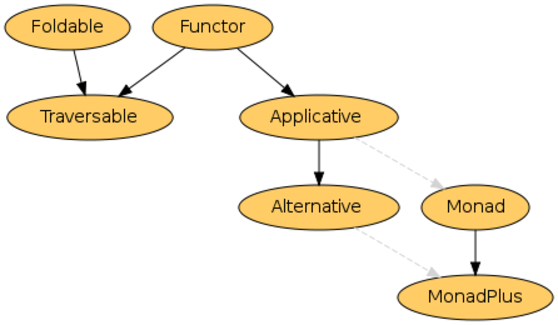
\includegraphics[scale = 0.7]{FunctorHierarchy.png}
\caption{Functor Hierarchy \cite{website:foldablenadtraversable}}
\label{fig:Functor Hierarchy}
\end{figure}

The \Verb!Functor! and \Verb!Foldable! instances providing functions for applying map-reduce to the data structure. The primary issue is that at the end
of the operation the structure if the data type is lost which would not help our cause since the result of a query must be a list of
substitutions which are essential pairs of language variable with language values(language constructs).

Enter, \Verb[formatcom=\bf]!Traversable!, %}{
it allows reduce whilst preserving the shape of the structure. Lastly, the Applicative instance is an intermediate
between a functor and a monad.

We create the necessary instances\endnote{%
  I am deeply suspicious of the instance for \texttt{Applicative} given.

  I agree, I think I just created one for the purpose of the diagram.
}
as shown in Figure~\ref{tab:flat-term-class-inst}.
\begin{code-list}
  \begin{minted}[linenos,gobble=4]{haskell}
    instance Functor (FlatTerm) where
      fmap = T.fmapDefault

    instance Foldable (FlatTerm) where
      foldMap = T.foldMapDefault

    instance Traversable (FlatTerm) where
       traverse f (Struct atom x)   =   Struct atom <$>
          sequenceA (Prelude.map f x)
       traverse _ (Var v)   =   pure (Var v)
       traverse _ Wildcard  =   pure (Wildcard)
       traverse _ (Cut i)   =    pure (Cut i)

    instance Applicative (FlatTerm) where
       pure x = Struct "" [x]
       _ <*> Wildcard  =   Wildcard
       _ <*> (Cut i)   =   Cut i
       _ <*> (Var v)   =   (Var v)
       (Struct a fs) <*> (Struct b xs)
                       = Struct (a ++ b) [f x | f <- fs, x <- xs]
  \end{minted}
  \caption{FlatTerm class instances}
  \label{tab:flat-term-class-inst}
\end{code-list}

The above lay the foundation to work with the library.
Coming back to the library, the language must have the \Verb!Unifiable! instance.
This works in tandem with the \Verb!UTerm! data type.
The \Verb!UTerm! data type captures the recursive structure of logic terms i.e, given some functor \(t\) which describes the
constructors of our logic terms, and some type \(v\) which describes our logic variables, the type
\Verb!UTerm! \(t\) \(v\) is the
type of logic terms: trees with multiple layers of \(t\) structure and leaves of type \(v\).
The \Verb!Unifiable! class gives one step of the unification process.
Just as we only need to specify one level of the ADT (i.e., \Verb!T!) and then we can use the library's \Verb!UTerm! to generate
the recursive ADT, so too we only need to specify one level of the unification (i.e., \Verb!zipMatch!) and then we can use
the library's operators to perform the recursive unification, subsumption.
This is shown in Figure~\ref{tab:zipMatch}.
\begin{code-list}
  \begin{minted}[linenos]{haskell}
    instance Unifiable (FlatTerm) where
       zipMatch (Struct al ls) (Struct ar rs) =
         if (al == ar) && (length ls == length rs)
         then Struct al <$>
           pairWith (\l r -> Right (l,r)) ls rs
         else Nothing
       zipMatch Wildcard _ = Just Wildcard
       zipMatch _ Wildcard = Just Wildcard
       zipMatch (Cut i1) (Cut i2) = if (i1 == i2)
         then Just (Cut i1)
         else Nothing
  \end{minted}
  \vspace*{-0.5\baselineskip}
  \caption{FlatTerm instance of zipMatch}
  \label{tab:zipMatch}
\end{code-list}

\paragraph{Logic Variables}
Unification involves side effects of binding logic variables to terms. To allow and keep track of these effects we use the Binding Monad
which provides facilities to generate fresh logic variables and perform look ups on dictionaries. By default two logic variable
implementations exist,\endnote{%
  In this immediate region, I (dgc) removed text inserted by a failed push or pull merge.
  Check to see that it is correct, or reverse commit \texttt{95804e3\dots}.
}

\begin{enumerate}
\item The IntVar implementation uses Int as the names of variables, and uses an
IntMap to keep track of the environment.

\item The STVar implementation uses STRefs, so we can use actual mutation for binding logic variables,
rather than keeping an explicit environment around.

\end{enumerate}

\begin{comment}
The library ships with two implementations of logic variables. The IntVar implementation uses Int as the names of variables, and uses an
IntMap to keep track of the environment. The STVar implementation uses STRefs, so we can use actual mutation for binding logic variables,
rather than keeping an explicit environment around. This implementation uses STVars.

Performing unification has the side effect of binding logic variables to terms. Thus, we'll want to use a monad in order to keep track of
these effects. The BindingMonad type class provides the definition of what we need from our ambient monad. In particular, we need to be
able to generate fresh logic variables, to bind logic variables, and to lookup what our logic variables are bound to. The library provides
the necessary instances for both IntVar and STVar.

You can provide your own implementations of Variable and BindingMonad.
\end{comment}

\textbf{Some stuff about Meta syntactic variables can be put in here}

This implementation uses STVars but a custom implementation can be used inside the BindingMonad.
For our language expressions to be unifiable we must deal with the variables in the expressions being compared. For that we extract the
variables and then convert them into a dictionary consisting of a free
variable for each language variable as shown in Figure~\ref{tab:varsToDictM}.

\begin{code-list}
  \begin{minted}[linenos,gobble=2]{haskell}
  variableExtractor :: Fix FlatTerm -> [Fix FlatTerm]
  variableExtractor (Fix x) = case x of
     (Struct _ xs) ->   Prelude.concat $ Prelude.map variableExtractor xs
     (Var v)      ->   [Fix $ Var v]
     _         ->   []

  variableNameExtractor :: Fix FlatTerm -> [VariableName]
  variableNameExtractor (Fix x) = case x of
     (Struct _ xs)   -> Prelude.concat $ Prelude.map variableNameExtractor xs
     (Var v)         -> [v]
     _             -> []

  variableSet :: [Fix FlatTerm] -> S.Set (Fix FlatTerm)
  variableSet a = S.fromList a

  variableNameSet :: [VariableName] -> S.Set (VariableName)
  variableNameSet a = S.fromList a

  varsToDictM :: (Ord a, Unifiable t) =>
      S.Set a -> ST.STBinding s (Map a (ST.STVar s t))
  varsToDictM set = foldrM addElt Map.empty set where
    addElt sv dict = do
      iv <- freeVar
      return $! Map.insert sv iv dict
  \end{minted}
  \vspace*{-1.0\baselineskip}
  \caption{Creating a variable dictionary}
  \label{tab:varsToDictM}
\end{code-list}
A language to STVar dictionary is only one part of the unification procedure, the terms themselves should be made
compatible for the in built unify procedure to perform look ups for the variables in them.
The dictionary along with the fixed point version flattened of the term, as shown in Figure~\ref{tab:to-UTerm}.
%
\begin{code-list}
  \begin{minted}[linenos,gobble=2]{haskell}
  uTermify
    :: Map VariableName (ST.STVar s (FlatTerm))
    -> UTerm FlatTerm (ST.STVar s (FlatTerm))
    -> UTerm FlatTerm (ST.STVar s (FlatTerm))
  uTermify varMap ux = case ux of
    UT.UVar _                -> ux
    UT.UTerm (Var v)        -> maybe (error "bad map") UT.UVar $
                                 Map.lookup v varMap
    -- UT.UTerm t            -> UT.UTerm $! fmap (uTermify varMap)
    UT.UTerm (Struct a xs)   -> UT.UTerm $ Struct a $!
                                         fmap (uTermify varMap) xs
    UT.UTerm (Wildcard)      -> UT.UTerm Wildcard
    UT.UTerm (Cut i)         -> UT.UTerm (Cut i)

  translateToUTerm ::
      Fix FlatTerm -> ST.STBinding s
              (UT.UTerm (FlatTerm) (ST.STVar s (FlatTerm)),
               Map VariableName (ST.STVar s (FlatTerm)))
  translateToUTerm e1Term = do
    let vs = variableNameSet $ variableNameExtractor e1Term
    varMap <- varsToDictM vs
    let t2 = uTermify varMap . unfreeze $ e1Term
    return (t2,varMap)
  \end{minted}
  \caption{Conversion to UTerm}
  \label{tab:to-UTerm}
\end{code-list}
%
and for later use to convert them back, as shown in Figure~\ref{tab:from-UTerm}.
%
\begin{code-list}
  \begin{minted}[linenos,gobble=2]{haskell}
  vTermify :: Map Int VariableName ->
              UT.UTerm (FlatTerm) (ST.STVar s (FlatTerm)) ->
              UT.UTerm (FlatTerm) (ST.STVar s (FlatTerm))
  vTermify dict t1 = case t1 of
    UT.UVar x  -> maybe (error "logic") (UT.UTerm . Var) $
                           Map.lookup (UT.getVarID x) dict
    UT.UTerm r ->
      case r of
        Var iv   -> t1
        _         -> UT.UTerm . fmap (vTermify dict) $ r

  translateFromUTerm ::
      Map VariableName (ST.STVar s (FlatTerm)) ->
      UT.UTerm (FlatTerm) (ST.STVar s (FlatTerm)) -> Prolog
  translateFromUTerm dict uTerm =
    P .  maybe (error "Logic") id . freeze . vTermify varIdDict $ uTerm where
      rot3 f a k v = f k v a
      inserter k v = Map.insert (UT.getVarID v) k
      forKV dict initial fn = Map.foldlWithKey' (rot3 fn) initial dict
      varIdDict = forKV dict Map.empty inserter
  \end{minted}
  \caption{Conversion from UTerm}
  \label{tab:from-UTerm}
\end{code-list}

\clearpage
The variable dictionaries and UTermified language expressions are unified in the binding monad as shown in Figure~\ref{tab:unification} and Figure~\ref{tab:unif-driver}.
%
\begin{code-list}
\begin{minted}[linenos]{haskell}
  monadicUnification ::
  (BindingMonad FlatTerm (STVar s FlatTerm) (ST.STBinding s))
  => (forall s. ((Fix FlatTerm) -> (Fix FlatTerm)
  ->  ErrorT (UT.UFailure (FlatTerm) (ST.STVar s (FlatTerm)))
             (ST.STBinding s) (UT.UTerm (FlatTerm) (ST.STVar s (FlatTerm)),
                               Map VariableName (ST.STVar s (FlatTerm)))))
monadicUnification t1 t2 = do
--  let
--    t1f = termFlattener t1
--    t2f = termFlattener t2
  (x1,d1) <- lift . translateToUTerm $ t1
  (x2,d2) <- lift . translateToUTerm $ t2
  x3 <- U.unify x1 x2
  --get state from somehwere, state -> dict
  return $! (x3, d1 `Map.union` d2)
\end{minted}
  \vspace*{-1.0\baselineskip}
  \caption{Unification code}
  \label{tab:unification}

\begin{minted}[linenos]{haskell}
goUnify ::
  (forall s. (BindingMonad FlatTerm (STVar s FlatTerm) (ST.STBinding s))
  =>
      (ErrorT
          (UT.UFailure FlatTerm (ST.STVar s FlatTerm))
          (ST.STBinding s)
          (UT.UTerm FlatTerm (ST.STVar s FlatTerm),
             Map VariableName (ST.STVar s FlatTerm)))
     )
  -> [(VariableName, Prolog)]
goUnify test = ST.runSTBinding $ do
  answer <- runErrorT $ test --ERROR
  case answer of
    (Left _)            -> return []
    (Right (_, dict))   -> f1 dict
\end{minted}
  \vspace*{-1.0\baselineskip}
  \caption{Driver code}
  \label{tab:unif-driver}
\end{code-list}


The final reconversion to return a list of substitutions,
  called \texttt{f1} in Figure~\ref{tab:unif-driver}, is shown in
  Figure~\ref{tab:vars-extract}.
\begin{code-list}
  \begin{minted}[linenos,gobble=2]{haskell}
  f1 ::
    (BindingMonad FlatTerm (STVar s FlatTerm) (ST.STBinding s))
    => (forall s. Map VariableName (STVar s FlatTerm)
        -> (ST.STBinding s [(VariableName, Prolog)])
       )
  f1 dict = do
    let ld1 = Map.toList dict
    ld2 <- Control.Monad.Error.sequence
           [ v1 | (k,v) <- ld1, let v1 = UT.lookupVar v]
    let ld3 = [ (k,v) | ((k,_),Just v) <- ld1 `zip` ld2]
        ld4 = [ (k,v) | (k,v2) <- ld3,
                let v = translateFromUTerm dict v2 ]
    return ld4
  \end{minted}
  \vspace*{-1.0\baselineskip}
  \caption{Variable substitution list extraction}
  \label{tab:vars-extract}
\end{code-list}

\begin{comment}

\section{Black box}


\section{Something about unification-fd and Monadic Unification}
Library \cite{unification-fd-lib}


Tutorial 1 \cite{website:unification-fd-lib-tutorial1}


Tutorial 2 \cite{website:unification-fd-lib-tutorial2}


\begin{enumerate}
\item What library provides ?

This module provides first-order structural unification over general structure types. It also provides the standard suite of functions
accompanying unification (applying bindings, getting free variables, etc.).

The implementation makes use of numerous optimization techniques. First, we use path compression everywhere (for weighted path compression
see Control.Unification.Ranked). Second, we replace the occurs-check with visited-sets. Third, we use a technique for aggressive
opportunistic observable sharing; that is, we track as much sharing as possible in the bindings (without introducing new variables), so
that we can compare bound variables directly and therefore eliminate redundant unifications.


\item Unifiable stuff

The basic class for generating, reading, and writing to bindings stored in a monad. These three functionalities could be split apart, but are combined in order to simplify contexts. Also, because most functions reading bindings will also perform path compression, there's no way to distinguish \yyy{"}{``}true\yyy{"}{''} mutation from mere path compression.

The superclass constraints are there to simplify contexts, since we make the same assumptions everywhere we use BindingMonad.


In order to use our T data type with the rest of the API, we'll need to give a Unifiable instance for it. Before we do that we'll have to give Functor, Foldable, and Traversable instances. These are straightforward and can be automatically derived with the appropriate language pragmas.

The Unifiable class gives one step of the unification process. Just as we only need to specify one level of the ADT (i.e., T) and then we can use the library's UTerm to generate the recursive ADT, so too we only need to specify one level of the unification (i.e., zipMatch) and then we can use the library's operators to perform the recursive unification, subsumption, etc.

The zipMatch function takes two arguments of type t a. The abstract t will be our concrete T type. The abstract a is polymorphic, which ensures that we can't mess around with more than one level of the term at once. If we abandon that guarantee, then you can think of it as if a is UTerm T v. Thus,t a means T (UTerm T v); and T (UTerm T v) is essentially the type UTerm T v with the added guarantee that the values aren't in fact variables. Thus, the arguments to zipMatch are non-variable terms.

The zipMatch method has the rather complicated return type: Maybe (t (Either a (a,a))). Let's unpack this a bit by thinking about how
unification works. When we try to unify two terms, first we look at their head constructors. If the constructors are different, then the
terms aren't unifiable, so we return Nothing to indicate that unification has failed. Otherwise, the constructors match, so we have to
recursively unify their subterms. Since the T structures of the two terms match, we can return Just t0 where t0 has the same T structure as
both input terms. Where we still have to recursively unify subterms, we fill t0 with Right(l,r) values where l is a subterm of the left
argument to zipMatch and r is the corresponding subterm of the right argument. Thus, zipMatch is a generalized zipping function for
combining the shared structure and pairing up substructures. And now, the implementation:

\begin{minted}[linenos]{haskell}

instance Unifiable T where
    zipMatch (T m ls) (T n rs)
        | m /= n    = Nothing
        | otherwise =
            T n <$> pairWith (\l r -> Right(l,r)) ls rs
\end{minted}
Where list-extras:Data.List.Extras.Pair.pairWith is a version of zip which returns Nothing if the lists have different lengths. So, if the
names m and n match, and if the two arguments have the same number of subterms, then we pair those subterms off in order; otherwise, either
the names or the lengths don't match, so we return Nothing.


\item UTerm stuff

The type of terms generated by structures t over variables v. The structure type should implement Unifiable and the variable type should
implement Variable.

The Show instance doesn't show the constructors, in order to improve legibility for large terms.

All the category theoretic instances (Functor, Foldable, Traversable,...) are provided because they are often useful; however, beware that
since the implementations must be pure, they cannot read variables bound in the current context and therefore can create incoherent
results. Therefore, you should apply the current bindings before using any of the functions provided by those classes.


\item STVar stuff

This module defines an implementation of unification variables using the ST monad.



\item IntVar stuff


This module defines a state monad for functional pointers represented by integers as keys into an IntMap. This technique was independently
discovered by Dijkstra et al. This module extends the approach by using a state monad transformer, which can be made into a backtracking
state monad by setting the underlying monad to some MonadLogic (part of the logict library, described by Kiselyov et al.).

Atze Dijkstra, Arie Middelkoop, S. Doaitse Swierstra (2008) Efficient Functional Unification and Substitution, Technical Report
UU-CS-2008-027, Utrecht University.

Oleg Kiselyov, Chung-chieh Shan, Daniel P. Friedman, and Amr Sabry (2005) Backtracking, Interleaving, and Terminating Monad Transformers,
ICFP

A \yyy{"}{``}mutable\yyy{"}{''} unification variable implemented by an integer. This provides an entirely pure alternative to truly mutable alternatives (like
STVar), which can make backtracking easier.

N.B., because this implementation is pure, we can use it for both ranked and unranked monads.

\item Binding Monad Stuff

A monad for handling STVar bindings.

Run the ST ranked binding monad. N.B., because STVar are rank-2 quantified, this guarantees that the return value has no such references.
However, in order to remove the references from terms, you'll need to explicitly apply the bindings and ground the term.

\item U.unify stuff

Unify two terms, or throw an error with an explanation of why unification failed. Since bindings are stored in the monad, the two input
terms and the output term are all equivalent if unification succeeds. However, the returned value makes use of aggressive opportunistic
observable sharing, so it will be more efficient to use it in future calculations than either argument.

\item U.unifyOccurs

A variant of unify which uses occursIn instead of visited-sets. This should only be used when eager throwing of occursFailure errors is
absolutely essential (or for testing the correctness of unify). Performing the occurs-check is expensive. Not only is it slow, it's
asymptotically slow since it can cause the same subterm to be traversed multiple times.

\clearpage

\item Translation stuff

\begin{code-list}
\begin{minted}[linenos,frame=single]{haskell}
monadicUnification :: (BindingMonad FlatTerm (STVar s FlatTerm) (ST.STBinding s)) => (forall s. ((Fix FlatTerm) -> (Fix FlatTerm) ->
  ErrorT (UT.UFailure (FlatTerm) (ST.STVar s (FlatTerm)))
           (ST.STBinding s) (UT.UTerm (FlatTerm) (ST.STVar s (FlatTerm)),
            Map VariableName (ST.STVar s (FlatTerm)))))
monadicUnification t1 t2 = do
--  let
--    t1f = termFlattener t1
--    t2f = termFlattener t2
  (x1,d1) <- lift . translateToUTerm $ t1
  (x2,d2) <- lift . translateToUTerm $ t2
  x3 <- U.unify x1 x2
  --get state from somehwere, state -> dict
  return $! (x3, d1 `Map.union` d2)


goUnify ::
  (forall s. (BindingMonad FlatTerm (STVar s FlatTerm) (ST.STBinding s))
  =>
      (ErrorT
          (UT.UFailure FlatTerm (ST.STVar s FlatTerm))
          (ST.STBinding s)
          (UT.UTerm FlatTerm (ST.STVar s FlatTerm),
             Map VariableName (ST.STVar s FlatTerm)))
     )
  -> [(VariableName, Prolog)]
goUnify test = ST.runSTBinding $ do
  answer <- runErrorT $ test --ERROR
  case answer of
    (Left _)            -> return []
    (Right (_, dict))   -> f1 dict


f1 ::
  (BindingMonad FlatTerm (STVar s FlatTerm) (ST.STBinding s))
  => (forall s. Map VariableName (STVar s FlatTerm)
      -> (ST.STBinding s [(VariableName, Prolog)])
     )
f1 dict = do
  let ld1 = Map.toList dict
  ld2 <- Control.Monad.Error.sequence [ v1 | (k,v) <- ld1, let v1 = UT.lookupVar v]
  let ld3 = [ (k,v) | ((k,_),Just v) <- ld1 `zip` ld2]
      ld4 = [ (k,v) | (k,v2) <- ld3, let v = translateFromUTerm dict v2 ]
  return ld4
\end{minted}
  \vspace*{-1.0\baselineskip}
  \caption{A sample Minted figure}
  \label{fig:sample}
\end{code-list}

\end{enumerate}
\end{comment}

\clearpage
\section{Chapter Recap}

\if\jobname={thesis-solanki}\else
\begin{scope}
  \nolinenumbers
  \enotesize
  \par
  \begin{singlespace}
  \setlength{\parskip}{12pt plus 2pt minus 1pt}
  \theendnotes
  \par
  \end{singlespace}
\end{scope}
\fi

\end{document}
